\documentclass[11pt, a4paper, oneside]{Thesis} % Paper size, default font size and one-sided paper
\usepackage{wrapfig}
\usepackage{lscape}
\usepackage{rotating}
\usepackage{graphicx}
\usepackage{caption}
\usepackage{amsmath}

% TikZ for flow diagrams
\usepackage{tikz}
\usetikzlibrary{arrows.meta, positioning, shapes.geometric, calc}


%\usepackage{subcaption} %incompatible with subfig
\usepackage[square, numbers]{natbib} % Use the natbib reference package - read up on this to edit the reference style; if you want text (e.g. Smith et al., 2012) for the in-text references (instead of numbers), remove 'numbers' v

\hypersetup{urlcolor=black, colorlinks=true} % Colors hyperlinks in blue - change to black if annoyingv`	
\title{\ttitle} % Defines the thesis title - don't touch this





%======================================================================|
%\thesistitle{An Approach to Writing a Thesis\\[3mm] for MDes at IIITDM}
\thesistitle{Hospital Management System}
\degree{B.Tech. Computer Science and Engineering}
\authors{Chakala Karthik \\[-2mm] (Roll No: 123cs0038) \\ \vspace{2mm}
G Deepak Desai \\[-2mm] (Roll No: 123cs0033) \\ \vspace{2mm}
Shaik Venkat \\[-2mm] (Roll No: 123cs0037) \\ \vspace{2mm}
N Bhargav Reddy \\[-2mm] (Roll No: 123cs0014) \\ \vspace*{1cm}
Under the Guidance of \\ Dr. V.S.R Krishnaiah \\ Department of CSE, IIITDM Kurnool}
\supervisor{Dr. V.S.R Krishnaiah}
\department{Department of CSE}
%======================================================================|


\tolerance=1
\emergencystretch=\maxdimen
\hyphenpenalty=10000
\hbadness=10000


%======================================================================|
\begin{document}
\makeatletter
\renewcommand*{\NAT@nmfmt}[1]{\textsc{#1}}
\makeatother

% prints author names as small caps


\frontmatter % Use roman page numbering style (i, ii, iii, iv...) for the pre-content pages

\setstretch{1.6} % Line spacing of 1.6 (double line spacing)

% Define the page headers using the FancyHdr package and set up for one-sided printing
\fancyhead{} % Clears all page headers and footers
\rhead{\thepage} % Sets the right side header to show the page number
\lhead{} % Clears the left side page header

\pagestyle{fancy} % Finally, use the "fancy" page style to implement the FancyHdr headers

\newcommand{\HRule}{\rule{\linewidth}{0.5mm}} % New command to make the lines in the title page

% PDF meta-data
\hypersetup{pdftitle={\ttitle}}
\hypersetup{pdfsubject=\subjectname}
\hypersetup{pdfauthor=\authornames}
\hypersetup{pdfkeywords=\keywordnames}

%----------------------------------------------------------------------------------------
%	TITLE PAGE
%----------------------------------------------------------------------------------------

\begin{titlepage}
\begin{center}


%\HRule \\[0.4cm] % Horizontal line
\vspace{0.4cm} % Horizontal line
{\huge \bfseries \ttitle}\\[0.4cm] % Thesis title
%\HRule \\[1.5cm] % Horizontal line
\vspace{1.5cm} % Horizontal line

 
\large \textit{A report submitted in partial fulfilment of the requirements\\ for the award of the degree of \\ B.Tech Computer Science and Engineering}\\[0.3cm] % University requirement text
\textit{by}\\[0.4cm]

\authornames

\vfill
\graphicspath{ {./Figures/} }
\begin{figure}[hb]
  \centering
  \includegraphics[width=0.3\linewidth]{klogo.png}
\end{figure}

\DEPTNAME\\ % Research group name and department name
\textsc{ \UNIVNAME}\\[1.5cm] % University name
\large \today\\[2cm] % Date


\end{center}

\end{titlepage}

%----------------------------------------------------------------------------------------
%	DECLARATION PAGE
%	Your institution may give you a different text to place here
%----------------------------------------------------------------------------------------


\Declaration{\addtocontents{toc}{\vspace{1em}} % Add a gap in the Contents, for aesthetics


%\begin{center}
%\LARGE{\underline{\textbf{Declaration of Originality}}}
%\end{center}
\noindent We, \textbf{Chakala Karthik (123cs0038)}, \textbf{G Deepak Desai (123cs0033)}, \textbf{Shaik Venkat (123cs0037)}, and \textbf{N Bhargav Reddy (123cs0014)} hereby declare that 
the material presented in the Project Report titled \textbf{Hospital Management System} 
\noindent represents original work carried out by us in the \textbf{Department of Computer Science and Engineering} at the \textbf{Indian Institute of Information Technology Design and Manufacturing Kurnool} during the years \textbf{2023 - 2024}.
%\noindent 
With my signature, I certify that:
\begin{itemize}
	\item I have not manipulated any of the data or results.\\[-10mm]
	\item I have not committed any plagiarism of intellectual
	property.
	I have clearly indicated and referenced the contributions of
		others.\\[-10mm]
	\item I have explicitly acknowledged all collaborative research
		and discussions.\\[-10mm]
	\item I have understood that any false claim will result in severe
		disciplinary action.\\[-10mm]
	\item I have understood that the work may be screened for any form
		of academic {misconduct}.
\end{itemize}

\vspace{10mm}

\noindent {\footnotesize{Date:	\hfill	Student's Signature}} \qquad

\vspace{10mm}

\noindent 

In my capacity as supervisor of the above-mentioned work, I certify
that the work presented in this Report is carried out under my supervision, and is 
worthy of consideration for the requirements of B.Tech.\ Project work.  

\vspace{10mm}

\noindent  {\footnotesize{Advisor's Name: Dr. V.S.R Krishnaiah \hfill Advisor's Signature}} \qquad

\vfill{}}

\clearpage % Start a new page

%----------------------------------------------------------------------------------------
%	ACKNOWLEDGEMENTS
%----------------------------------------------------------------------------------------

\setstretch{1.3} % Reset the line-spacing to 1.3 for body text (if it has changed)

\acknowledgements{\addtocontents{toc}{\vspace{1em}} % Add a gap in the Contents, for aesthetics

I would extend my sincerest gratitude...

}
\clearpage % Start a new page

%----------------------------------------------------------------------------------------
%	LIST OF CONTENTS/FIGURES/TABLES PAGES
%----------------------------------------------------------------------------------------

\pagestyle{fancy} % The page style headers have been "empty" all this time, now use the "fancy" headers as defined before to bring them back

\lhead{\emph{Contents}} % Set the left side page header to "Contents"
\tableofcontents % Write out the Table of Contents

%----------------------------------------------------------------------------------------
%	DEDICATION
%----------------------------------------------------------------------------------------
%
\setstretch{1.3} % Return the line spacing back to 1.3
%
\pagestyle{empty} % Page style needs to be empty for this page
%
\dedicatory{Dedicated to Dr. V.S.R Krishnaiah} % Dedication text
%
\addtocontents{toc}{\vspace{2em}} % Add a gap in the Contents, for aesthetics

%----------------------------------------------------------------------------------------
%THESIS CONTENT - CHAPTERS
%----------------------------------------------------------------------------------------
\mainmatter % Begin numeric (1,2,3...) page numbering
\pagestyle{fancy} 


\chapter{Introduction} 
\label{Chapter1} 
\lhead{Chapter 1. \emph{Introduction}} 

\section{Background and Motivation}

Modern hospitals operate a complex ecosystem of services across outpatient care, inpatient admissions, diagnostics, pharmacy, billing, and telemedicine. Many institutions still rely on siloed tools or manual workflows that lead to appointment clashes, delayed communication, and scattered patient records. This project addresses those gaps by designing and implementing a comprehensive Hospital Management System (HMS) that unifies administrative, clinical, and financial workflows in a single platform.

The system offers secure authentication, a patient portal with appointment booking and history, a doctor workspace, real-time chat, and virtual consultations via WebRTC. Operational modules include laboratory and pharmacy workflows, EMR integration, billing and payments (Razorpay), home visits, and a robust admin analytics dashboard for decision-making. The goal is to provide a cohesive, privacy-conscious, and scalable solution that reduces administrative friction and improves patient outcomes.

Technically, the HMS uses a modern full‑stack architecture: Next.js (React + TypeScript) and Tailwind CSS on the frontend for responsive, accessible UI; Node.js/Express on the backend; and Supabase (Postgres) for secure, relational data. JWT underpins authentication and authorization; Nodemailer powers email notifications; Razorpay enables online payments; and WebRTC supports low-latency video for virtual appointments. Admin analytics are visualized using Recharts.

The expected outcomes include improved appointment utilization, faster triage, transparent billing, and actionable insights for administrators. The platform emphasizes auditability, role-based access control, and maintainability to support real-world deployment in clinics and mid-sized hospitals.

\subsection{Scope and Objectives}
Scope and objectives: The HMS covers core hospital workflows—registration, scheduling, EMR, diagnostics, pharmacy, billing, and analytics—while enabling remote care through chat and video. Key objectives are to streamline patient onboarding, reduce waiting times, centralize clinical data, automate notifications, and provide leadership with real-time insights.

The system is designed with security and compliance in mind: encrypted transport (HTTPS), hashed credentials, least-privilege access, and auditable actions. The modular architecture supports incremental rollout—departments can adopt features progressively without disrupting hospital operations.

\subsection{Contributions}
Contributions: We implement unified appointment management (in-person and virtual), department/doctor-wise analytics, and integrated billing. Reusable frontend components (DateFilter, ChartCard, StatCard) provide a consistent UX. Backend services expose RESTful APIs for patients, staff, doctors, and admins, backed by optimized Supabase queries.

\section{Report Organization}
Document organization: The report introduces the problem and goals, surveys related systems, presents the architecture and database design, details the implementation of each module, demonstrates analytics visualizations, and evaluates the system with tests and metrics. It concludes with limitations and future work, including advanced EMR features and predictive analytics.

Summary: The HMS delivers a secure, extensible platform that modernizes hospital workflows, improves coordination among stakeholders, and enhances patient experience through digital-first services.

This chapter frames the motivation, scope, and structure of the project report to guide the reader through the HMS design and implementation.

% Chapter Template

\chapter{Related Work and Requirements} % Main chapter title

\label{Chapter2} % Change X to a consecutive number; for referencing this chapter elsewhere, use \ref{Chapter2}

\lhead{Chapter 2. \emph{Related Work and Requirements}} % Change X to a consecutive number; this is for the header on each page - perhaps a shortened title

%----------------------------------------------------------------------------------------
%	SECTION 1
%----------------------------------------------------------------------------------------

\section{Related Systems and Literature}

This chapter surveys related systems and positions our Hospital Management System (HMS) within the broader landscape of clinical information systems. We examine appointment schedulers, EMR/EHR platforms, and telemedicine tools, highlighting the fragmentation that occurs when institutions combine disparate point solutions. Our HMS integrates these capabilities end-to-end to minimize context switching, reduce data duplication, and improve care coordination.

%-----------------------------------
%	SUBSECTION 1
%-----------------------------------
\subsection{Standards and Interoperability}
Open-source HMS options provide modular building blocks but often lack real-time communication and analytics. Enterprise suites deliver breadth but are costly and rigid. Standards such as HL7/FHIR inform data exchange, yet practical interoperability remains challenging for mid-sized hospitals. Our approach balances pragmatism and standards alignment—Supabase (Postgres) for structured data, REST APIs for service boundaries, and exportable reports for integration.

%-----------------------------------
%	SUBSECTION 2
%-----------------------------------

\subsection{Key Differentiators}
Key differentiators of our HMS include unified appointment management (in-person and virtual via WebRTC), role-based workspaces for patients, doctors, staff, and admins, and a first-class analytics experience using Recharts. We emphasize maintainable TypeScript codebases on both frontend and backend, auditable actions, and secure authentication with JWT.

%----------------------------------------------------------------------------------------
%	SECTION 2
%----------------------------------------------------------------------------------------

\section{Functional and Non-Functional Requirements}
Requirements distilled from the survey include: centralized appointment scheduling, integrated EMR and diagnostics, streamlined billing with online payments, secure communication (chat and video), and actionable admin analytics. Non-functional goals prioritize security, privacy, reliability, scalability, and usability suited to clinic and hospital settings. 
% Chapter Template

\chapter{System Architecture and Database Design} % Main chapter title

\label{Chapter3} % Change X to a consecutive number; for referencing this chapter elsewhere, use \ref{Chapter3}

\lhead{Chapter 3. \emph{System Architecture and Database Design}} % Change X to a consecutive number; this is for the header on each page - perhaps a shortened title

%----------------------------------------------------------------------------------------
%	SECTION 1
%----------------------------------------------------------------------------------------

\section{System Architecture Overview}

System architecture: The HMS follows a modular, service-oriented design. The frontend is built with Next.js (React + TypeScript) and Tailwind CSS for responsive UI. The backend uses Node.js/Express with RESTful endpoints grouped by role (patient, doctor, staff, admin). Supabase (Postgres) provides secure relational storage and row-level filters. Authentication and authorization use JWT; emails are sent via Nodemailer; Razorpay powers payments; WebRTC enables real-time video for virtual appointments.

%-----------------------------------
%	SUBSECTION 1
%-----------------------------------
\subsection{Backend Services and APIs}
Backend services and APIs: Endpoints are organized under `/api/patient`, `/api/doctor`, `/api/staff`, and `/api/admin`. Middleware handles JWT verification and role checks. Appointment flows unify in-person and virtual visits; billing integrates at booking and service completion. Analytics endpoints under `/api/admin/analytics/*` aggregate revenue, visits, and performance with date filters and grouping.

%-----------------------------------
%	SUBSECTION 2
%-----------------------------------

\subsection{Database Design}
Database design: Core tables include `User`, `Patient`, `Doctor`, `Staff`, `Appointments`, `VirtualAppointments`, `Billing`, `Departments`, `LabTests`, `Pharmacy`, `HomeVisit`, `EMR`, and `AuditLogs`. Foreign keys link patients and doctors to appointments and bills; status fields capture workflow state; timestamps support analytics windows and auditing.

%----------------------------------------------------------------------------------------
%	SECTION 2
%----------------------------------------------------------------------------------------

\section{Deployment and Configuration}
Deployment and configuration: Environment variables define endpoints and URLs (e.g., \texttt{NEXT\_PUBLIC\_BACKEND\_BASE\_URL} for the frontend and \texttt{FRONTEND\_BASE} for backend-generated links). The system supports local development with hot reload and can be containerized for production. Logging and error handling surface actionable diagnostics without leaking sensitive data.
% Chapter Template

\chapter{Implementation: Patient Workflows} % Main chapter title

\label{Chapter4} % Change X to a consecutive number; for referencing this chapter elsewhere, use \ref{Chapter4}

\lhead{Chapter 4. \emph{Implementation: Patient Workflows}} % Change X to a consecutive number; this is for the header on each page - perhaps a shortened title

%----------------------------------------------------------------------------------------
%	SECTION 1
%----------------------------------------------------------------------------------------

\section{Patient-Facing Implementation Overview}

Implementation overview: We implemented patient-facing workflows including appointment discovery, booking, and management. The patient dashboard exposes quick actions, including a “View Appointments” card linking to upcoming bookings. The appointments page fetches scheduled visits, supports cancel/reschedule, and hides the booking form in view-only mode using a `mode=view` query parameter. Email notifications are sent on booking and changes.

%-----------------------------------
%	SUBSECTION 1
%-----------------------------------
\subsection{Frontend Flows}
Frontend flows: Built with Next.js and Tailwind CSS. Reusable components manage loading states and accessibility. Client code calls backend APIs via Axios, using \texttt{NEXT\_PUBLIC\_BACKEND\_BASE\_URL}. State management relies on React hooks; UI provides responsive cards, tables, and dialogs for cancel/reschedule with clear feedback.

%-----------------------------------
%	SUBSECTION 2
%-----------------------------------

\subsection{Backend Services}
Backend services: Express routes under `/api/patient/appointments/*` unify read and write flows, with JWT middleware enforcing access. Nodemailer sends confirmations and changes; cancellation and rescheduling trigger appropriate updates and emails. Virtual appointments include WebRTC links built from \texttt{FRONTEND\_BASE}, ensuring correct meeting URLs.

%----------------------------------------------------------------------------------------
%	SECTION 2
%----------------------------------------------------------------------------------------

\section{Security and Reliability}

Security and reliability: Requests use HTTPS and JWT; sensitive IDs are server-resolved where possible. Error handling returns actionable messages and preserves invariant checks (ownership, valid status transitions). Logging enables traceability without exposing PHI, and rate-limiting is applied to sensitive endpoints as needed. 
% Chapter Template

\chapter{Admin Analytics and Reporting} % Main chapter title

\label{Chapter5} % Change X to a consecutive number; for referencing this chapter elsewhere, use \ref{Chapter5}

\lhead{Chapter 5. \emph{Admin Analytics and Reporting}} % Change X to a consecutive number; this is for the header on each page - perhaps a shortened title

%----------------------------------------------------------------------------------------
%	SECTION 1
%----------------------------------------------------------------------------------------

\section{Admin Analytics Overview}

Admin analytics and reporting: The HMS provides an analytics dashboard for administrators to monitor revenue, patient visits, and staff performance. Views include revenue by department and service category, visit volumes by department and doctor, and staff productivity by role. Filters support daily, weekly, monthly, yearly, and custom ranges to enable trend analysis and operational decision-making.

%-----------------------------------
%	SUBSECTION 1
%-----------------------------------
\subsection{Frontend Analytics UI}
Frontend analytics UI: Implemented in Next.js with Recharts. The dashboard uses tabs to switch between Revenue, Departments, Doctors, and Staff. Reusable components—`DateFilter`, `ChartCard`, and `StatCard`—ensure consistent presentation and responsive layouts. Data is fetched via Axios from \texttt{NEXT\_PUBLIC\_BACKEND\_BASE\_URL}, with loading states and error fallbacks for reliability.

%-----------------------------------
%	SUBSECTION 2
%-----------------------------------

\subsection{Backend Analytics Services}
Backend analytics services: Express routes under `/api/admin/analytics/*` aggregate revenue from `Billing`, visit counts from `Appointments` and `VirtualAppointments`, and staff metrics from operational tables. Date filters are passed as `from`/`to` and applied in Supabase queries. Service classification tags include Virtual Consultation and Inpatient where applicable. Results are grouped by department, doctor, and role for chart-ready responses.

%----------------------------------------------------------------------------------------
%	SECTION 2
%----------------------------------------------------------------------------------------

\section{Security and Performance}

Security and performance: Admin endpoints are protected with JWT and role checks, restricting access to administrators. Queries are shaped to minimize payloads and leverage database filtering and grouping. Responses support pagination where necessary, and errors return actionable messages. Future optimizations include caching frequently requested ranges and pre-aggregations for monthly reports. 
% Chapter Template

\chapter{Testing and Evaluation} % Main chapter title

\label{Chapter6} % Change X to a consecutive number; for referencing this chapter elsewhere, use \ref{Chapter6}

\lhead{Chapter 6. \emph{Testing and Evaluation}} % Change X to a consecutive number; this is for the header on each page - perhaps a shortened title

%----------------------------------------------------------------------------------------
%	SECTION 1
%----------------------------------------------------------------------------------------

\section{Testing Strategy and Coverage}

Testing and evaluation: We validated the HMS through unit tests, integration tests, and scenario-driven end-to-end checks. Backend routes were exercised with authenticated requests covering appointment creation, cancellation, rescheduling, billing generation, and analytics queries. Frontend workflows were tested for accessibility, error states, and responsive behavior across breakpoints.

%-----------------------------------
%	SUBSECTION 1
%-----------------------------------
\subsection{Backend API Testing}
Backend testing: API integration tests verified JWT protection, role-based access (patient, doctor, staff, admin), and validation for required fields. Appointment flows were tested for consistency across in-person and virtual visits; billing hooks were asserted for correct creation and totals. Analytics endpoints were validated for date filtering, grouping, and inclusion of virtual consultations and inpatient services.

%-----------------------------------
%	SUBSECTION 2
%-----------------------------------

\subsection{Frontend and Performance}
Frontend and performance: UI paths for booking, viewing, canceling, and rescheduling were exercised with mocked network conditions. Recharts visualizations were checked for correctness under different date ranges and empty states. Basic performance checks ensured acceptable response times for core routes under typical loads; logs and error boundaries were verified to provide actionable diagnostics without leaking sensitive data.

%----------------------------------------------------------------------------------------
%	SECTION 2
%----------------------------------------------------------------------------------------

\section{Results and Discussion}

Results and discussion: Tests confirmed that authentication, role checks, and core patient/admin workflows behave as expected. Analytics charts render consistently across date windows, and appointment management provides clear user feedback. Limitations include the absence of automated load testing and partial coverage of edge cases (e.g., concurrent edits), which are reserved for future work alongside CI/CD hardening and observability. 
% Chapter Template

\chapter{Conclusion and Future Work} % Main chapter title

\label{Chapter7} % Change X to a consecutive number; for referencing this chapter elsewhere, use \ref{Chapter7}

\lhead{Chapter 7. \emph{Conclusion and Future Work}} % Change X to a consecutive number; this is for the header on each page - perhaps a shortened title

%----------------------------------------------------------------------------------------
%	SECTION 1
%----------------------------------------------------------------------------------------

\section{Conclusion}

Conclusion: This project delivers a full‑stack Hospital Management System that unifies patient, doctor, staff, and admin workflows. Core contributions include secure authentication, unified appointment management (in‑person and virtual), EMR-linked operational modules (lab, pharmacy, inpatient, home visits), and an analytics dashboard for revenue, visits, and staff performance. The implementation emphasizes security, usability, and maintainability with a modern TypeScript codebase and well‑structured REST APIs backed by Supabase.

%-----------------------------------
%	SUBSECTION 1
%-----------------------------------
\subsection{Outcomes and Impact}
Outcomes and impact: The HMS reduces administrative overhead through centralized scheduling and billing, improves communication with chat and video, and equips administrators with actionable insights. Reusable components and clear service boundaries accelerate future development and institutional adoption.

%-----------------------------------
%	SUBSECTION 2
%-----------------------------------

\subsection{Limitations}
Limitations: Load testing and advanced observability are out of scope; interoperability is limited to exports rather than live HL7/FHIR exchange; and predictive analytics are not yet implemented. These constraints inform the roadmap for future enhancements.

%----------------------------------------------------------------------------------------
%	SECTION 2
%----------------------------------------------------------------------------------------

\section{Future Work}

Future work: Key extensions include HL7/FHIR-based interoperability, advanced EMR features (order sets, allergies, medication reconciliation), automated reminders and escalation policies, comprehensive load testing and SLOs, mobile apps for patients and clinicians, and machine‑learning‑assisted analytics for demand forecasting and triage support. 

% Project features and TikZ diagrams
\chapter{Complete Feature Documentation}
\label{chap:features}

\lhead{Chapter 8. \emph{Complete Feature Documentation}}

This chapter presents a consolidated, module-centric documentation of the Hospital Management System (HMS). It integrates system design, analysis, workflows, backend APIs, database entities, and UI behaviors across Patient, Doctor, Admin, and Staff roles. The objective is to provide a single, coherent view of the complete feature set implemented in the application.

\section{System Overview}
\subsection{Architecture}
\begin{itemize}
  \item \textbf{Frontend}: Next.js (TypeScript, React), TailwindCSS, Recharts; JWT stored in browser storage; calls backend REST APIs.
  \item \textbf{Backend}: Node.js (TypeScript), Express, Socket.IO (chat), Nodemailer (email), Razorpay (payments), in-memory signaling for WebRTC.
  \item \textbf{Database}: Supabase (PostgreSQL) with Row-level security managed by backend; joins across \texttt{User}, \texttt{Patient}, \texttt{Doctor}, \texttt{Appointments}, \texttt{VirtualAppointments}, \texttt{Billing}, \texttt{Departments}, \texttt{LabTests}, \texttt{Pharmacy}, \texttt{HomeVisit}, \texttt{EMR}, \texttt{AuditLogs}, etc.
  \item \textbf{Deployment}: Local dev on \texttt{http://localhost:3000} (frontend) and \texttt{http://localhost:5000} (backend). Env-based base URLs for building links.
\end{itemize}

\subsection{Cross-cutting Concerns}
\begin{itemize}
  \item \textbf{Authentication}: JWT with role claims (admin, doctor, patient, staff); protected routes enforce role-based authorization.
  \item \textbf{Validation}: Request payload validation at route-handlers; defensive checks for IDs, dates, and status transitions.
  \item \textbf{Auditing}: Selected actions recorded in \texttt{AuditLogs} and available in admin audit screens.
  \item \textbf{Notifications}: Email (Nodemailer) for confirmations, reminders, lab results, invitations.
\end{itemize}

\section{Authentication and Role-Based Access}
\subsection{Purpose}
Secure system entry and controlled access to features and data.
\subsection{Technologies}
Express middleware (\texttt{protect}), JWT, Supabase user records.
\subsection{Key APIs}
\begin{itemize}
  \item \texttt{POST /api/auth/login} (returns JWT with role)
  \item \texttt{GET /api/admin/profile}, \texttt{/api/doctor/profile}, \texttt{/api/patient/profile} (role-gated)
\end{itemize}
\subsection{Database Tables}
\texttt{User} (role), \texttt{Patient}, \texttt{Doctor}, \texttt{Staff}.
\subsection{UI Workflow}
\begin{verbatim}
Login -> Verify credentials -> Issue JWT -> Store -> Redirect to role dashboard
Admin -> /dashboard/admin | Doctor -> /dashboard/doctor | Patient -> /dashboard/patient
\end{verbatim}
\subsection{Permissions}
\begin{itemize}
  \item Admin: full administrative features, analytics, settings.
  \item Doctor: own appointments, EMR, chat, virtual consult.
  \item Patient: booking, history, billing, chat, virtual consult.
  \item Staff: reception (appointments), pharmacy, lab modules.
\end{itemize}

\section{Appointment Management}
\subsection{Purpose}
Enable patients to book, cancel, or reschedule appointments with doctors; allow doctors/staff to manage status.
\subsection{Technologies}
Next.js UI, Express routes, Supabase joins.
\subsection{Key APIs}
\begin{itemize}
  \item \texttt{GET /api/patient/appointments/departments}
  \item \texttt{GET /api/patient/appointments/doctors/:departmentId}
  \item \texttt{GET /api/patient/appointments/times/:doctorId/:date}
  \item \texttt{POST /api/patient/appointments} (book \& auto-bill paid)
  \item \texttt{GET /api/patient/appointments/upcoming} (normalized list)
  \item \texttt{PATCH /api/patient/appointments/:type/:id/cancel}
  \item Staff daily view: \texttt{GET /api/staff/appointments/today}
\end{itemize}
\subsection{Database Tables}
\texttt{Appointments}, \texttt{Doctor}, \texttt{Patient}, \texttt{Billing}, \texttt{Departments}.
\subsection{UI Workflow}
\begin{verbatim}
Patient: Select Dept -> Select Doctor -> Pick Date/Time -> Pay -> Confirm
Doctor: View schedule -> Complete visits -> Update status
Staff: View day sheet -> Check-in/No-Show/Completed
\end{verbatim}
\subsection{Role Permissions}
Patients can create/cancel own bookings; Doctors update status of own appointments; Staff manage schedule logistics.

\subsection{Appointment Flow (Diagram)}
\begin{verbatim}
[Patient] --selects--> [Department] --chooses--> [Doctor] --picks--> [Slot]
   |                             |                         |
   +-----> [POST /appointments] --(create)--> [Appointments + Billing]
                                       |
                                 [Email/SMS confirm]
\end{verbatim}

\section{Virtual Consultation (WebRTC)}
\subsection{Purpose}
Real-time video consultations between patient and doctor.
\subsection{Technologies}
WebRTC (browser), custom signaling (Express endpoints), email invitation, Socket endpoints not mandatory for signaling.
\subsection{Key APIs}
\begin{itemize}
  \item Signaling: \texttt{/api/video/room/:id (GET/POST/DELETE)} for offer/answer/candidates
  \item Invite: \texttt{POST /api/video/invite} -> sends meeting link to patient \& doctor
\end{itemize}
\subsection{Database Tables}
\texttt{VirtualAppointments} (date, time, doctor, patient, status, optional link), \texttt{Doctor}, \texttt{Patient}.
\subsection{UI Workflow}
\begin{verbatim}
Patient pays -> Creates virtual appt -> Invite email -> Join /video/:roomId at time
Doctor receives email -> Joins room -> Conducts consultation
\end{verbatim}
\subsection{Permissions}
Only participants (patient/doctor) can access the room link; URL points to frontend site.

\section{Chat System}
\subsection{Purpose}
Asynchronous messaging between patient and doctor for pre/post consultation clarifications.
\subsection{Technologies}
Socket.IO for real-time events, REST for history.
\subsection{Database Tables}
\texttt{ChatMessages}, \texttt{User} (by role), mapping tables for participants if present.
\subsection{UI/Flow (Diagram)}
\begin{verbatim}
[User] --connects--> [Socket.IO] --join room--> [patient_doctor_room]
   |                                         |
 send message ------------------------------->|-- store & broadcast --> peers
\end{verbatim}
\subsection{Permissions}
Only assigned/related users can join corresponding rooms.

\section{Notifications}
\subsection{Purpose}
Keep users informed: booking confirmations, reminders, lab results, virtual consult invites.
\subsection{Technologies}
Nodemailer (SMTP), scheduled jobs for reminders.
\subsection{Key APIs}
\begin{itemize}
  \item \texttt{POST /api/video/invite} (emails both patient \& doctor)
  \item Reminder jobs: appointment, virtual appointment, home visit
\end{itemize}
\subsection{Database}
Reads from \texttt{Appointments}, \texttt{VirtualAppointments}, \texttt{HomeVisit}, and user email fields via joins.

\section{Pharmacy Module}
\subsection{Purpose}
Dispense prescriptions and generate associated bills.
\subsection{Technologies}
Staff UI (pharmacist), Express routes, Supabase.
\subsection{Key APIs}
\begin{itemize}
  \item \texttt{GET /api/staff/pharmacy/pending} (appointments awaiting dispensing)
  \item \texttt{PUT /api/staff/pharmacy/dispense/:appointmentId} (marks dispensed and creates bill)
  \item \texttt{GET /api/staff/pharmacy/medicines} (catalog)
\end{itemize}
\subsection{Database Tables}
\texttt{Appointments}, \texttt{EMR} (prescriptions), \texttt{Billing}, \texttt{Pharmacy}, \texttt{Patient}, \texttt{Doctor}.
\subsection{UI Workflow}
\begin{verbatim}
Pharmacist: Pending -> View latest EMR -> Dispense -> Auto-generate Bill (Unpaid)
Patient: Pays later via billing module; receives receipt email on payment
\end{verbatim}
\subsection{Permissions}
Pharmacist (staff role) only; enforced via middleware (role check).

\section{Laboratory Module}
\label{sec:laboratory-module}
\subsection{Purpose}
Track tests, submit results, notify patients.
\subsection{Technologies}
Staff UI (lab), Express, Supabase joins to \texttt{TestsCatalog}, \texttt{Patient->User}.
\subsection{Key APIs}
\begin{itemize}
  \item \texttt{GET /api/staff/lab/pending}
  \item \texttt{PUT /api/staff/lab/result/:testId} (submit results and email patient)
  \item \texttt{GET /api/staff/lab/samples}
\end{itemize}
\subsection{Database Tables}
\texttt{LabTests} (with \texttt{test\_catalog\_id}), \texttt{Patient}, \texttt{User}, \texttt{Billing} (diagnostics revenue), \texttt{TestsCatalog}.
\subsection{UI Workflow}
\begin{verbatim}
Lab: Pending list -> Enter results -> Mark Completed -> Email patient w/ result summary
\end{verbatim}
\subsection{Permissions}
Lab staff only; results append to patient record context.

\section{Billing and Payments}
\subsection{Purpose}
Record service charges, mark payment status, generate receipts.
\subsection{Technologies}
Razorpay for online payment (where used), Nodemailer for receipts, Express routes.
\subsection{Key APIs}
\begin{itemize}
  \item \texttt{GET /api/patient/bills} (list)
  \item \texttt{PUT /api/patient/bills/:billId/pay} (mark Paid; send receipt)
  \item Auto-billing on booking: \texttt{POST /api/patient/appointments} inserts a Paid consultation bill
\end{itemize}
\subsection{Database Tables}
\texttt{Billing} (\texttt{total\_amount}, \texttt{status}, \texttt{payment\_date}, \texttt{payment\_method}), \texttt{Appointments}, \texttt{Patient}.
\subsection{UI Workflow}
\begin{verbatim}
Patient: View bills -> Pay -> Email receipt
Staff/Modules: Create bills (dispense, inpatient, home visit) -> Patients settle later
\end{verbatim}
\subsection{Permissions}
Patients can view/pay own bills; staff can create module-driven bills (pharmacy, inpatient, home visit).

\section{Home Visit}
\subsection{Purpose}
Book at-home healthcare services (Doctor/Nurse/Physiotherapist/Caregiver), optionally assign doctor.
\subsection{Technologies}
Express routes, email confirmation, dedicated table.
\subsection{Key APIs}
\begin{itemize}
  \item \texttt{POST /api/home-visit/create-bill} (pre-payment bill)
  \item \texttt{POST /api/home-visit} (booking)
  \item \texttt{GET /api/home-visit} (filters: patient, assigned, service type)
  \item \texttt{PATCH /api/home-visit/:id} (status/assignment)
\end{itemize}
\subsection{Database Tables}
\texttt{HomeVisit} (\texttt{service\_type}, \texttt{assigned\_id}, \texttt{visit\_date/time}, \texttt{status}), \texttt{Patient}, \texttt{Doctor}.
\subsection{UI Workflow}
\begin{verbatim}
Patient: Choose service -> Provide date/time/address -> (Optional) Assigned doctor -> Confirmation email
Admin/Coordinator: Update assignment/status as needed
\end{verbatim}

\section{Administrative Analytics and Dashboards}
\subsection{Purpose}
Provide revenue, patient visits, and staff activity insights with filters (day/week/month/year/custom).
\subsection{Technologies}
Backend aggregation endpoints (TypeScript + Supabase), Next.js UI with Recharts, Tailwind grid layout.
\subsection{Key APIs}
\begin{itemize}
  \item \texttt{GET /api/admin/analytics/revenue}
  \item \texttt{GET /api/admin/analytics/revenue/department}
  \item \texttt{GET /api/admin/analytics/patients/department}
  \item \texttt{GET /api/admin/analytics/patients/doctor}
  \item \texttt{GET /api/admin/analytics/staff/performance}
\end{itemize}
\subsection{Database Tables}
\texttt{Billing}, \texttt{Appointments}, \texttt{VirtualAppointments}, \texttt{Doctor}, \texttt{Departments}, \texttt{LabTests}.
\subsection{UI Workflow}
\begin{verbatim}
Filters (period/range) -> Fetch datasets -> Render charts (bar/line/pie/area)
Revenue by Dept | Trends over time | Top 10 busy doctors | Staff contribution
\end{verbatim}
\subsection{Analytics Flow (Diagram)}
\begin{verbatim}
[Admin UI] -> set filters -> call /api/admin/analytics/*
    -> aggregate in DB (GROUP BY, date filters) -> return chart-ready JSON
    -> render Recharts in responsive cards
\end{verbatim}

\section{Doctor Module}
\subsection{Purpose}
Manage schedules, complete appointments, update EMR, review chat, and join virtual consultations.
\subsection{Key APIs}
\begin{itemize}
  \item \texttt{GET /api/doctor/appointments}
  \item \texttt{PUT /api/doctor/appointments/:appointmentId/complete}
  \item \texttt{GET /api/doctor/patients}
\end{itemize}
\subsection{Database}
\texttt{Appointments}, \texttt{EMR}, \texttt{Patient->User} joins.
\subsection{UI Workflow}
\begin{verbatim}
Doctor: View upcoming -> Complete visits -> EMR notes -> Respond to chat -> Join /video/:id
\end{verbatim}

\section{Patient Module}
\subsection{Purpose}
Self-service booking, medical history, billing, chat, and virtual consult access.
\subsection{Key APIs}
\begin{itemize}
  \item \texttt{GET /api/patient/medical-history}
  \item \texttt{GET /api/patient/bills}, \texttt{PUT /api/patient/bills/:billId/pay}
  \item \texttt{GET /api/patient/appointments/upcoming}
\end{itemize}
\subsection{Database}
\texttt{EMR}, \texttt{Billing}, \texttt{Appointments}, \texttt{VirtualAppointments}.
\subsection{UI Workflow}
\begin{verbatim}
Patient: Dashboard -> Book/Manage appointments -> Pay bills -> Join virtual consult -> Chat
\end{verbatim}

\section{Staff Module}
\subsection{Purpose}
Operational functions for receptionists, pharmacists, and laboratorists.
\subsection{Key APIs}
\begin{itemize}
  \item Reception: \texttt{GET /api/staff/appointments/today}, \texttt{PATCH /api/staff/appointments/:id/status}
  \item Pharmacy: see \S\ref{sec:pharmacy-module}
  \item Lab: see \S\ref{sec:laboratory-module}
\end{itemize}
\subsection{Database}
\texttt{Appointments}, \texttt{Billing}, \texttt{LabTests}, \texttt{Pharmacy}.

\section{Workflows (Detailed Diagrams)}
\subsection{Authentication Flow}
\begin{verbatim}
[User] -> /login -> POST /api/auth/login -> [JWT] -> store -> navigate to role dashboard
\end{verbatim}

\begin{figure}[htbp]
  \centering
  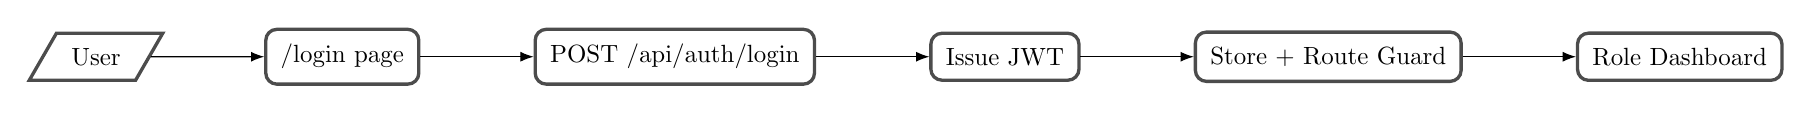
\begin{tikzpicture}[
    scale=0.9,
    every node/.style={transform shape},
    node distance=1.6cm,
    >=Latex,
    box/.style={rectangle, rounded corners, draw=black!70, fill=white, very thick, inner sep=6pt, align=center},
    io/.style={trapezium, trapezium left angle=60, trapezium right angle=120, draw=black!70, fill=white, very thick, inner sep=6pt, align=center}
  ]
    \node[io] (user) {User};
    \node[box, right=of user] (login) {/login page};
    \node[box, right=of login] (api) {POST /api/auth/login};
    \node[box, right=of api] (jwt) {Issue JWT};
    \node[box, right=of jwt] (guard) {Store + Route Guard};
    \node[box, right=of guard] (dash) {Role Dashboard};
    \draw[->] (user) -- (login);
    \draw[->] (login) -- (api);
    \draw[->] (api) -- (jwt);
    \draw[->] (jwt) -- (guard);
    \draw[->] (guard) -- (dash);
  \end{tikzpicture}
  \caption{Authentication flow \& route guarding}
  \label{fig:auth-flow}
\end{figure}
\subsection{Chat Flow}
\begin{verbatim}
[Client] --connect--> [Socket Server]
  |--join(room: patient_doctor)--> ok
  |--emit('message', payload)-----> [server saves & broadcasts] -> peers receive
\end{verbatim}

\begin{figure}[htbp]
  \centering
  
\begin{tikzpicture}[
    scale=0.9,
    every node/.style={transform shape},
    node distance=2cm,
    >=Latex,
    box/.style={rectangle, rounded corners, draw=black!70, fill=white, very thick, inner sep=6pt, align=center}
  ]
    \node[box] (c1) {Client (Patient)};
    \node[box, right=3cm of c1] (srv) {Socket.IO Server};
    \node[box, right=3cm of srv] (c2) {Client (Doctor)};
    \draw[->] (c1) -- node[above]{connect + join(room)} (srv);
    \draw[->] (c2) -- node[above]{connect + join(room)} (srv);
    \draw[<->, bend left=20] (c1) to node[above]{message events} (srv);
    \draw[<->, bend left=20] (srv) to node[above]{broadcast} (c2);
  \end{tikzpicture}
  \caption{Chat workflow via Socket.IO rooms}
  \label{fig:chat-flow}
\end{figure}
\subsection{Appointment Workflow}
\begin{verbatim}
Patient -> Dept -> Doctor -> Slot -> POST /appointments -> Billing (Paid)
Doctor -> Complete -> EMR update -> Follow-up chat if needed
\end{verbatim}

\begin{figure}[htbp]
  \centering
  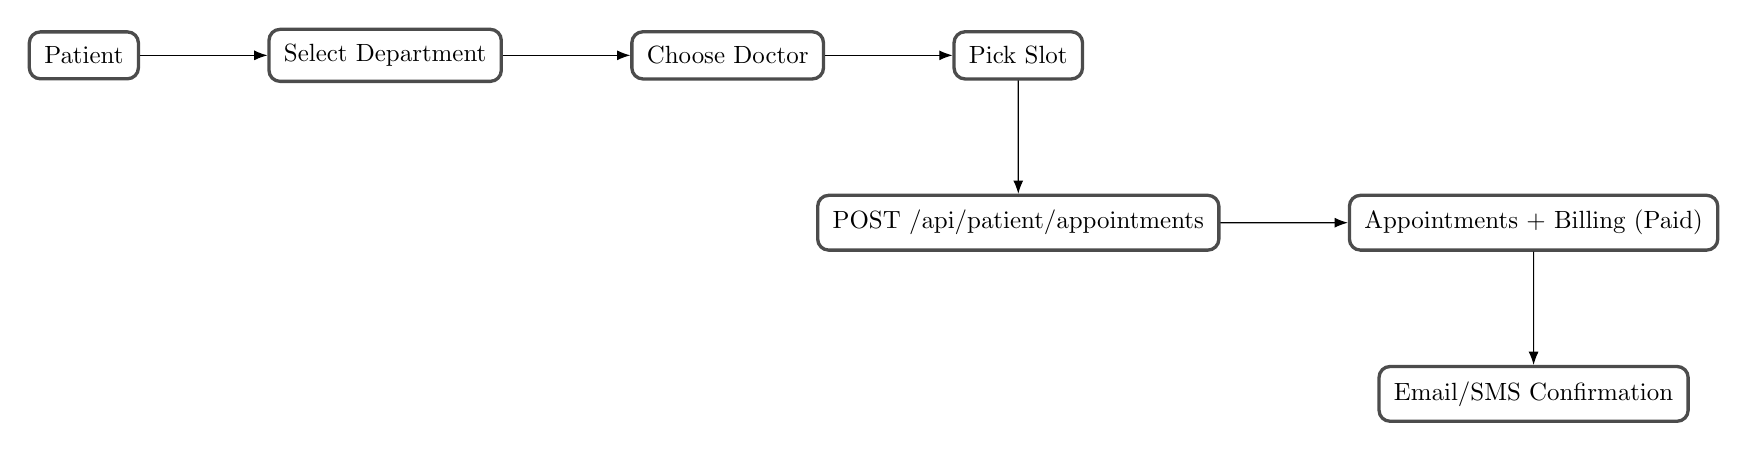
\begin{tikzpicture}[
    scale=0.9,
    every node/.style={transform shape},
    node distance=1.8cm,
    >=Latex,
    box/.style={rectangle, rounded corners, draw=black!70, fill=white, very thick, inner sep=6pt, align=center}
  ]
    \node[box] (pat) {Patient};
    \node[box, right=of pat] (dept) {Select Department};
    \node[box, right=of dept] (doc) {Choose Doctor};
    \node[box, right=of doc] (slot) {Pick Slot};
    \node[box, below=1.6cm of slot] (post) {POST /api/patient/appointments};
    \node[box, right=of post] (bill) {Appointments + Billing (Paid)};
    \node[box, below=1.6cm of bill] (email) {Email/SMS Confirmation};
    \draw[->] (pat) -- (dept);
    \draw[->] (dept) -- (doc);
    \draw[->] (doc) -- (slot);
    \draw[->] (slot) -- (post);
    \draw[->] (post) -- (bill);
    \draw[->] (bill) -- (email);
  \end{tikzpicture}
  \caption{End-to-end appointment booking flow}
  \label{fig:appt-flow}
\end{figure}
\subsection{Admin Analytics Workflow}
\begin{verbatim}
Admin picks period -> /api/admin/analytics/* -> Supabase aggregates -> Charts render
\end{verbatim}

\begin{figure}[htbp]
  \centering
  
\begin{tikzpicture}[
    node distance=2.2cm,
    >=Latex,
    box/.style={rectangle, rounded corners, draw=black!70, fill=white, very thick, inner sep=6pt, align=center}
  ]
    \node[box] (ui) {Admin UI (Filters)};
    \node[box, right=of ui] (api) {/api/admin/analytics/*};
    \node[box, right=of api] (agg) {Supabase Queries\newline (GROUP BY, date range)};
    \node[box, right=of agg] (chart) {Chart-ready JSON $\rightarrow$ Recharts};
    \draw[->] (ui) -- (api);
    \draw[->] (api) -- (agg);
    \draw[->] (agg) -- (chart);
  \end{tikzpicture}
  \caption{Analytics data flow from filters to charts}
  \label{fig:analytics-flow}
\end{figure}

\section{APIs Summary (Representative)}
\subsection{Public/Utility}
\texttt{/api (doctors list, video signaling endpoints)}
\subsection{Patient}
\texttt{/api/patient} (profile, appointments, medical-history, billing, chat, status, manage appointments)
\subsection{Doctor}
\texttt{/api/doctor} (profile, appointments, EMR, chat, uploads)
\subsection{Admin}
\texttt{/api/admin} (doctors, patients, staff, departments, settings, analytics, audit)
\subsection{Staff}
\texttt{/api/staff} (profile, lab, pharmacy, daily appointments, inventory)

\section{Database Entities (Selected)}
\begin{itemize}
  \item \textbf{User(user\_id, role, name, email, ...)} $\rightarrow$ links to \texttt{Patient}, \texttt{Doctor}, \texttt{Staff}.
  \item \textbf{Patient(patient\_id, user\_id, ...)}, \textbf{Doctor(doctor\_id, user\_id, department\_id, ...)}
  \item \textbf{Appointments(appointment\_id, patient\_id, doctor\_id, date, time, status)}
  \item \textbf{VirtualAppointments(virtual\_appointment\_id, patient\_id, doctor\_id, appointment\_date, appointment\_time, status)}
  \item \textbf{Billing(bill\_id, patient\_id, appointment\_id, services, total\_amount, status, payment\_date, payment\_method)}
  \item \textbf{Departments(department\_id, name)}, \textbf{LabTests(lab\_test\_id, test\_catalog\_id, status, ...)}
  \item \textbf{Pharmacy(pharmacy\_id, medicine\_details, price)}, \textbf{HomeVisit(visit\_id, service\_type, assigned\_id, visit\_date/time, status)}
  \item \textbf{EMR(...)} for clinical notes; \textbf{AuditLogs(...)} for admin audit views.
\end{itemize}

\section{Non-Functional Considerations}
\begin{itemize}
  \item \textbf{Performance}: DB filtering by indexed columns (dates, status, foreign keys); pagination on heavy lists.
  \item \textbf{Security}: JWT auth, role checks, parameter validation, hidden internal IDs in UI.
  \item \textbf{Reliability}: Email delivery errors are non-blocking; background jobs for reminders.
  \item \textbf{Scalability}: Analytics endpoints designed to return chart-ready minimal payloads.
\end{itemize}

\section{Conclusion}
This chapter consolidates the HMS features as implemented across UI, API, and database layers. It is intended as a single reference for reviewers to understand module purpose, flows, technologies, and data touchpoints without duplicating the detailed content present in other chapters.


%----------------------------------------------------------------------------------------
%THESIS CONTENT - APPENDICES
%----------------------------------------------------------------------------------------
% Removed Appendices per project requirement

\backmatter

%----------------------------------------------------------------------------------------
%BIBLIOGRAPHY
%----------------------------------------------------------------------------------------
% Removed Bibliography per project requirement

\end{document}  
